\section{Architecture}
%       - Give a name of your solution:  \gls{ndn} virtual function based 
% planning for interoperable \gls{pid} (?)

%       - Explain its components: 1)  interoperable \gls{pid} / \gls{ndn} mapping 
% function? 2) \gls{ndn} planner, 3) \gls{ndn} controller? .....

%       - Sequence diagram: how they interact

\label{planning-ndn}
% add planning and need for interoperability
% refer to the section where deployment is actually done
% include interoperability part in illustration
% dus architecture gaat over de componenten, waarom we dat zo doen, op basis van diagrams, echt de architecture planning dus 

This section will discuss the method we used in order to plan an \gls{ndn} with scalability in mind. Scalability is defined as capacity to be changed in size or scale. In order to plan an \gls{ndn} with this goal in mind we will use a combination of McCabe's method (section \ref{overview-mccabe}) and \gls{tosca} (section \ref{overview-tosca}). McCabe will function as a method to guide design choices with scalability and performance requirements in mind. While \gls{tosca} will function as an implementation method that provides the means to control the whole life cycle of the network design and deployment. Furthermore, a proof of concept will be discussed that we implemented in a limited scope, in order to proof the method in practice.


\subsection{Design requirements and analysis (McCabe)}
\label{planning-requirements}
In this section we will apply McCabe's approach in order to establish the design requirements and analyze the properties of \gls{ndn} and how it can be applied to solve the problem stated from section \ref{introduction-background}. As discussed in section \ref{introduction-ndn} and \ref{introduction-related-work}, \gls{ndn} is designed to make a distribution network possible and is gaining popularity in big science. Another requirement is flexible scalability, this will be addressed by deploying and managing \gls{ndn} in an NVF-style. Therefore, \gls{ndn} will be deployed as virtual functions and managed centrally via virtualization techniques as discussed in section \ref{overview-virtualization}. The first step is to make an overview of the requirements and known \gls{ndn} scalability and performance issues.

The following analysis is based on the design requirements and will provide a baseline for the high-level network design. As discussed in the related work (section \ref{introduction-related-work}), several key scalability and performance metrics were addressed. Several NDN-specific design choices need to be made. These include the consideration that \gls{ndn} is an overlay, on top of e.g. IP. Within this context it was concluded that TCP provided the most satisfying performance when compared to UDP. Furthermore, there are several \gls{ndn} strategies to choose from. The 'leave copy everywhere' cache decision strategy and the 'least recently used' cache replacement strategy were considered to be the overall best performing choices. However, for the forward strategies there was no decisive conclusion on which a selection could be based on. Therefore, we will use the default forwarding strategy; best-route. In terms of cache size, Koulouzis et al. recommends a cache size twice the size of the largest data object residing in the used repositories. The performance configurations mentioned can be configured in the \texttt{nfd.conf} file of the NDN-CXX\footnote{\url{https://github.com/named-data/ndn-cxx}} application. \gls{cxx} is one of the most mature software implementations of \gls{ndn} and therefore used in our design. Other performance optimization solutions which were mentioned in the related work require changes in the source-code. These source-code optimizations were not made public.

Furthermore, for the following hardware requirements a baseline was determined based on the software documentation, the the problem statement from section \ref{introduction-background} and related work from section \ref{introduction-related-work}. For VM memory requirements, at least 12GB is recommended. This was determined based on the recommended system requirements for Kubernetes \cite{kubernetes-system-requirements} and the fact that the use case will be I/O intensive. Therefore, I/O caching in memory benefits performance. In order to have sufficient disk space to cache \gls{ndn} data objects, install software, store logs and containers, a minimum of 100GB of storage is recommended as a baseline. Based on related work, a minimum of 4 CPU cores (Xeon) running at 2.0GHz is recommended when an average throughput of 10Gbps is required.

% eerste zin moet concreter, waarom is die interoperability nodig?
% design komt nog niet ter sprake, dus niet 'we will propose a design'
%

Due to the use of NDN, we need interoperability of \glspl{pid} with the \gls{ndn} namespace. For 
We will propose a design, which achieves \gls{pid} interoperability with the \gls{ndn} namespace and makes it feasible to add future \gls{pid} types.



Our design is based on related work done by Karakannas \cite{icn-bd}, by avoiding the \gls{pid} to \gls{ndn} translation on client side \cite{icn-bd}. The pattern matching method was based on related work by Mousa for identifying different \gls{pid} type schemas \cite{ndn-app-aware}. The research done by Olschanowsky et. al. was used for deriving \gls{ndn} names from metadata \cite{ndn-man}.
We will reimplement the principles of \gls{naas4pid} in order to demonstrate the \gls{pid} interoperability extensibility feature.
We combine the aforementioned related work and extended it with an extendable interoperability feature. The proposed design for our solution will be further discussed in \ref{planning-deploying}.
Our design adheres to the following principles, which will be discussed in more detail in section \ref{pid-poc}.
 
\begin{itemize}
    \item{Translation is transparent to the user.}
    \item{Support for multiple \gls{pid} types.}
    \item{Extensible with future \gls{pid} types with different naming schemas.}
\end{itemize}

These principles are all functions within our design. In section \ref{planning-architecture}, we will discuss the components which are responsible for these functions.

\subsection{Architecture (McCabe)}
\label{planning-architecture}
With the design requirements established, we can develop a high-level network design. As mentioned in section \ref{overview-virtualization}, virtualization allows for flexible allocation of cloud resources via VMs while scalability of software applications can be realized by the use of containers in a NVF-style. If more cloud resources are required, then this can be done by deploying more VMs. Furthermore, if needed, VMs can be deployed in other geographically located cloud providers, expanding the data distribution availability. The virtual \gls{ndn} functions running inside these cloud providers, can then provide locally cached copies of data objects. And thus providing data distribution which lowers the chance of network congestion. In figure \ref{fig:high-level-network-design} we illustrate our high-level network design. In this illustration there are two conceptual cloud providers; 'mulhouse' and 'nimes'. In both of these cloud providers a VM is deployed in order to allocate resources.

\begin{figure}[H]
\centering
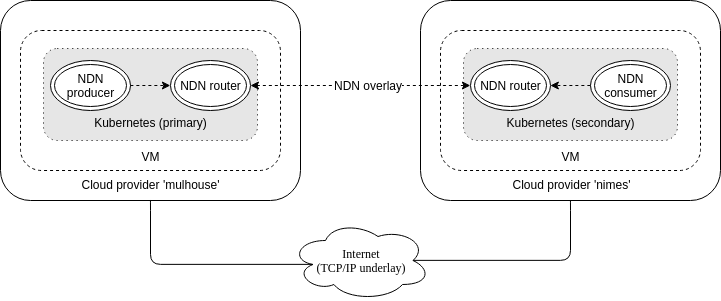
\includegraphics[width=\columnwidth]{Images/high-level-network-design.png}
\caption{High-level network design.}
\label{fig:high-level-network-design}
\end{figure}

Our high-level network design (figure \ref{fig:high-level-network-design}) contains three different virtual functions for \gls{ndn} nodes. The producer is assigned the function to make data available in the NDN. The consumer is assigned to request data from the producer. However, in NDN, any node that has named data, can reply to interest packets. So the producer and consumer functions can be interchangeable. The router's function is to forward interest packets between the two cloud providers. This forwarding is done in the \gls{ndn} overlay, which runs on top of the internet (underlay). These \gls{ndn} functions are deployed via a Kubernetes cluster (section \ref{overview-virtualization}), spread over the two conceptual cloud providers; ('mulhouse' and 'nimes'). These cloud providers are spread geographically in order to provide users with their regional \gls{ndn} cache. Kubernetes can be used to keep a central control over the NDN, where pods (containers) can be created, removed and managed. These pods are spawned from images and custom tailored for their specific network function. This is done by the use of scripts running inside the containers, which configure the \gls{ndn} based on environment variables provided by Kubernetes, as described in section \ref{overview-virtualization}. In summary; resources can be scaled in or out by deploying more VMs. In order to provide users a local \gls{ndn} cache, a regional cloud provider can be used to deploy a VM. By the use of Kubernetes, the \gls{ndn} application (node) can be scaled in and out as well. Where each \gls{ndn} node can be responsible for caching/forwarding a different subset of the naming hierarchy, in order to load-balance requests. However, cache misses are expensive since they require a rebuild of the cache, which puts load on the original publisher of the data, e.g. on SeaDataCloud. Which is what we want to prevent. Therefore, pods preferably are configured with persistent data volumes (section \ref{overview-virtualization}), on which the cached data can be stored outside of the container. Kubernetes can also load-balance requests between a set of identical pods. However, if these pods do not share the same persistent cached data, cache misses will occur, which results in performance degradation.

%At the 

As discussed in \ref{planning-requirements}, the functions we described need to be implemented in components. Our proposed design to be implemented in a proof of concept consists of the following components, each with their own functionality; the \gls{pid} server, the \gls{pid} to \gls{ndn} gateway and the client. In the high-level network design as illustrated in figure \ref{fig:high-level-network-design}, the client is interpreted as the consumer. The \gls{pid} server is interpreted as the producer, as long as the object is not already cached in NDN. Which then \gls{ndn} acts as the producer. The consumer retrieves the object via the IP underlay from the \gls{pid} server if the object is not cached in \gls{ndn} already. In our proof of concept, these components are conceptually part of the \gls{ndn} we have setup. The general idea is that a user enters a \gls{pid} of the object that the user want to retrieve at the client and gets back the requested object as shown in figure \ref{fig:sdc_model}. The retrieval of an object depends if the object is already published in the \gls{ndn} or not, which is further described in sections \ref{client} and \ref{gw}.



%\subsection{Design for \gls{pid} interoperability}
%In this section, we implemented the following in our proof of concept to answer our research question (section \ref{introduction-research-question}). We will propose a design, which achieves \gls{pid} interoperability with the \gls{ndn} namespace and makes it feasible to add future \gls{pid} types. Our design is based on related work done by Karakannas \cite{icn-bd}, by avoiding the \gls{pid} to \gls{ndn} translation on client side \cite{icn-bd}. The pattern matching method was based on related work by Mousa for identifying different \gls{pid} type schemas \cite{ndn-app-aware}. The research done by Olschanowsky et. al. was used for deriving \gls{ndn} names from metadata \cite{ndn-man}.
%We have reimplemented the principles of \gls{naas4pid} in order to demonstrate the \gls{pid} interoperability extensibility feature.
%We combined the aforementioned related work and extended it with an extendable interoperability feature. The proposed design for our solution is illustrated in figure \ref{fig:sdc_model}.
%Our design adheres to the following principles, which will be discussed in more detail in this section.
 
%\begin{itemize}
%    \item{Translation is transparent to the user.}
%    \item{Support for multiple \gls{pid} types.}
%    \item{Extensible with future \gls{pid} types with different naming schemas.}
%\end{itemize}

%\begin{figure}[H]
%\centering
%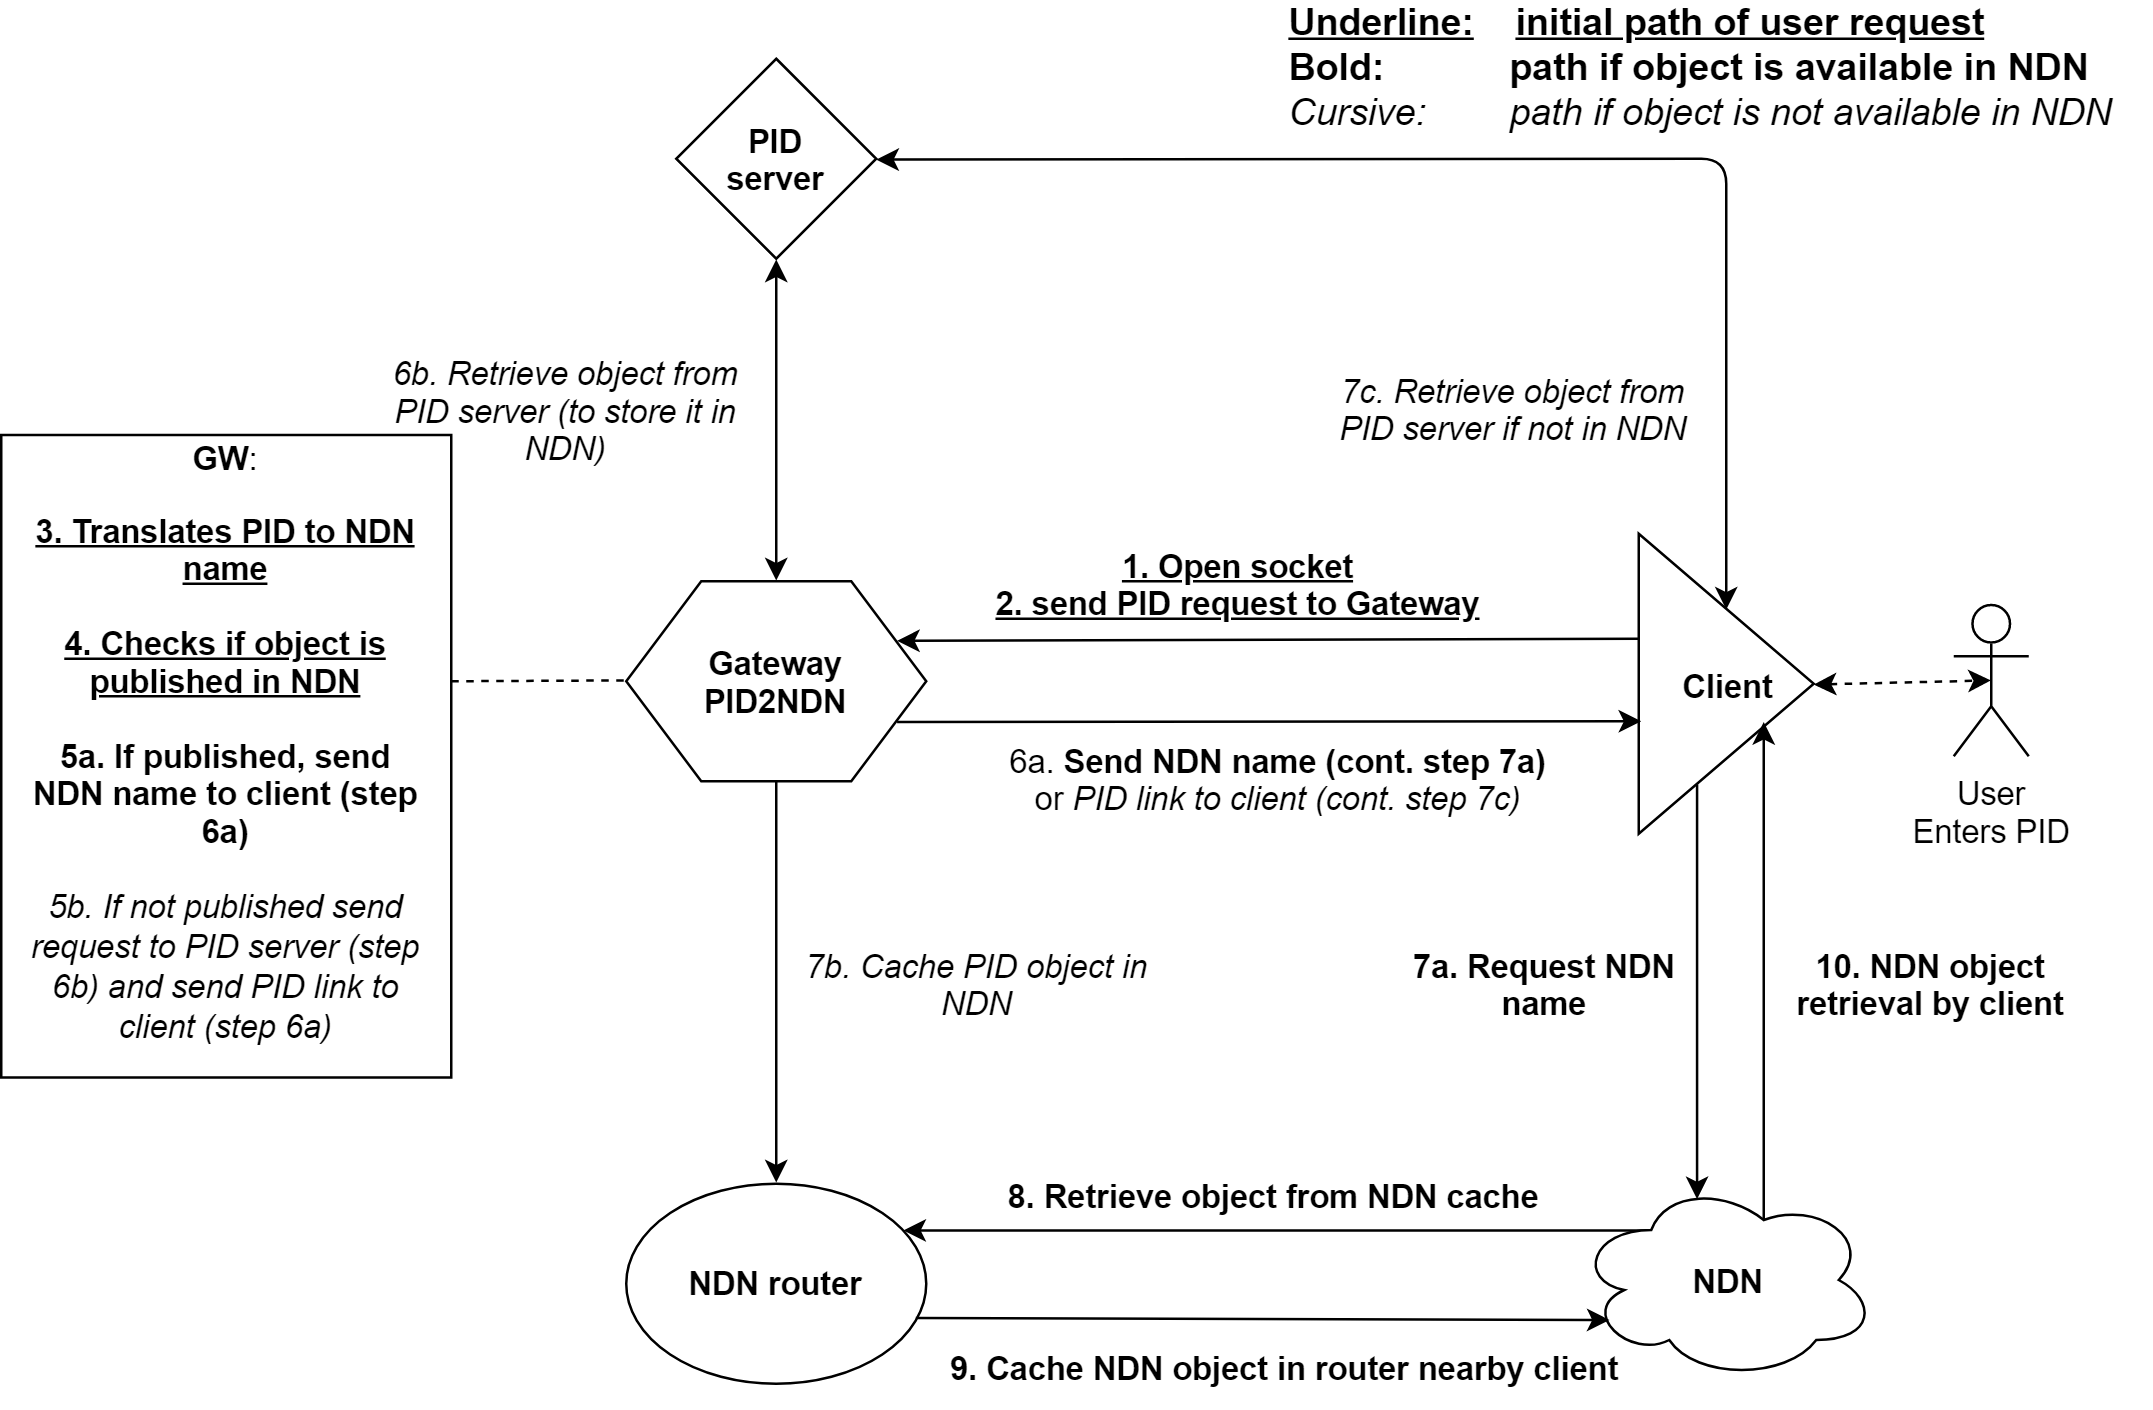
\includegraphics[width=\textwidth]{Images/PIDtoNDN10.png}
%\caption{NDN virtual function based 
%planning for achieving \gls{pid} interoperability}
%\label{fig:sdc_model}
%\end{figure}